%----------------------------------------------------------------------------
\section{SysML}\label{sec:sysml}
%----------------------------------------------------------------------------

SysML is a widely known and used Systems Modeling Language. Its aim is to provide a generic, extendable modeling language, capable of describing the most complicated systems from the specifications, all the way down to the actual behaviours of specific modules.

The previously introduced formal behaviour models have the power to describe many different behaviours a component may have, and are easy to reason about. However, such low-level models are not easy for users to write and maintain; that is why languages such as SysML exist - they provide high-level abstractions over low-level formal models.

In the following section I will present how SysML implements the two behaviour models introduced in \autoref{sec:behaviour_models}.

\subsection{State Machine}

State Machines are a high-level abstraction over deterministic finite state machines. Please note, that the exact semantics of SysML State Machines are not needed for this work, I only introduce the concept briefly for the possibly use-cases it has. A given state machine contains many \emph{states}, and \emph{transitions} between said states. Transitions use \emph{triggers} to enable them, and can also have an \emph{effect} on the component itself. Such an effect is called the \emph{action} of the transition. \autoref{fig:sysml_state_machine} is a simple example.

\begin{figure}[!ht]
	\centering
	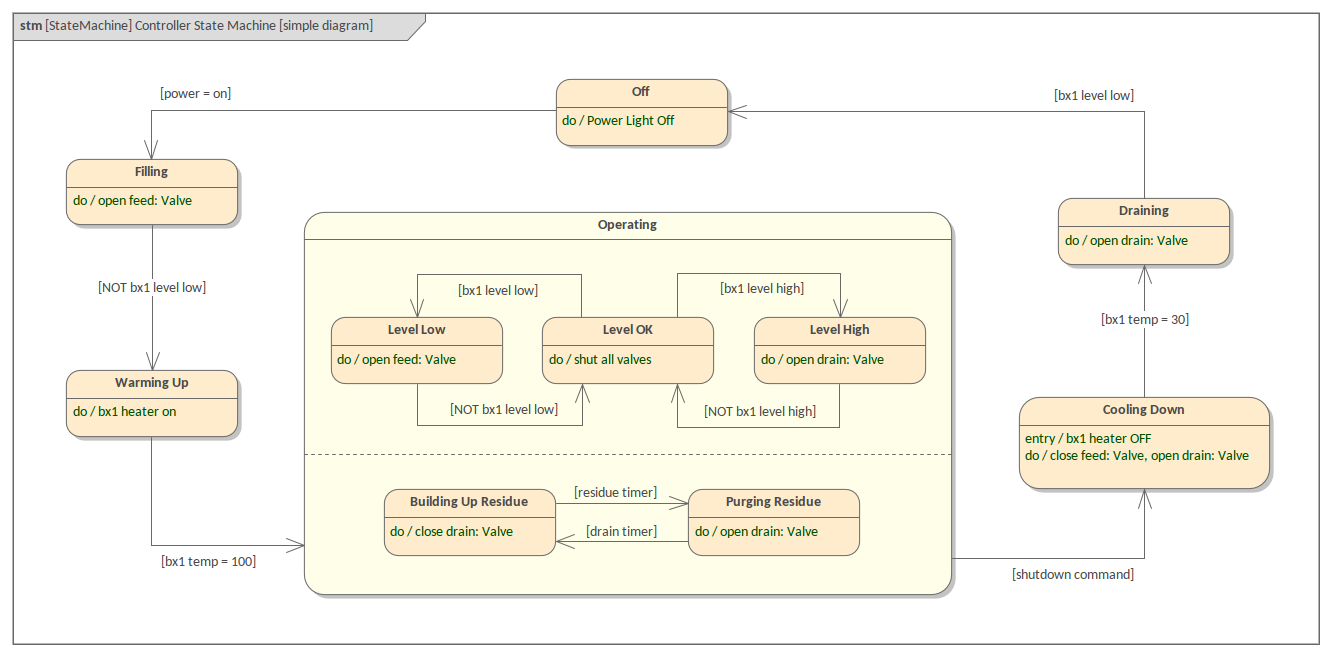
\includegraphics[width=67mm, keepaspectratio]{figures/sysml_state_machine.png}\hspace{1cm}
	\caption{A SysML State Machine.}
	\label{fig:sysml_state_machine}
\end{figure}

State Machines can also have \emph{composite} states and regions, which help with simplifying the behaviour model.

Along with actions defined on transitions, states may also have multiple actions associated with them. \emph{entry actions} defines a set of actions to be performed \emph{before} the state becomes the current state, \emph{exit actions} is a set of actions to be performed \emph{after} the state is no longer the current state. On a similar logic, \emph{do actions} is a set of actions to perform \emph{while} the state machine is in the given state. This fact will be address more in depth in \autoref{sec:gal_vs_sysml}. 

\subsection{Activity}

Activities are a high-level abstraction over Petri nets. In this section, I will introduce the semantics of Activities using Petri nets as formal semantics. Note however, since not all elements in SysML activity diagrams have execution semantics, I will only consider a set of the modeling elements, including basic actions, initial nodes, final nodes, join nodes, fork nodes, merge nodes, decision nodes, pins and object/control flows.\cite{fuml}\cite{https://doi.org/10.1002/sys.21524}

-- simple activity diagram --

\subsubsection*{Actions}

The specific operation an Action describes can be stated in various ways, usually in JavaScript or plain old English (Opaque action). In JavaScript, the engineer may access and change variables inside the containing object, send signals to connected objects, or just call existing functions.

-- example of action with js --

There are many different kinds of Activity Nodes, which describe different behaviour for guiding tokens through them.

\subsection{Combining Behaviours}

In SysML the behaviours can be combined using the Call Behaviour sintax, which means the semantics here is combined with the called behaviour's semantics. For example, a state machine's state may have a do action, in which a Call Behaviour action is specified. 